\documentclass[a4paper,11pt,twoside,titlepage,openright]{book}

\usepackage[english]{babel}
\usepackage{color}
\usepackage{graphicx}
\usepackage{amsmath}
\numberwithin{equation}{section}
\usepackage[margin=3cm]{geometry}
\usepackage{hyperref}
\usepackage{epsfig,amsfonts}
\usepackage{xcolor,import}


\pagestyle{plain}

\newcommand{\ud}[1]{\underline{#1}}
\newcommand{\e}[1]{\underline{e}_{#1}}
\newcommand{\lt}{\left}
\newcommand{\rt}{\right}
\DeclareMathOperator{\n}{\underline{n}}
\DeclareMathOperator{\ei}{\underline{e}_1}
\DeclareMathOperator{\et}{\underline{e}_2}
\DeclareMathOperator{\ex}{\underline{e}_x}
\DeclareMathOperator{\ey}{\underline{e}_y}
\DeclareMathOperator{\ez}{\underline{e}_z}
\DeclareMathOperator{\nin}{\underline{n}_{in}}
\DeclareMathOperator{\nout}{\underline{n}_{out}}
\DeclareMathOperator{\np}{\underline{n}_{P}}
\DeclareMathOperator{\bragg}{\theta_{bragg}}
\DeclareMathOperator{\DD}{\cos(\theta)^2 - \sin(\psi)^2}
\newcommand{\wdg}{\wedge}
\newcommand{\hypot}[1]{\textbf{\textcolor{green}{#1}}}


\begin{document}

\title{ToFu geometric tools\\ Intersection of a cone with a plane}
\author{Didier VEZINET}
\date{15.10.2019}
\maketitle

\tableofcontents

\chapter{Geometry}
\label{chap:Geometry}

\section{Generic cone and plane}

Let's consider a half-cone $C_1$ (defined only for $z > 0$), with summit on the cartesian frame's origin $(O, \ex, \ey, \ez)$.
The cone's axis is the $(O,\ez)$ axis.
It's angular half-opening is $\theta$.

Let's consider plane $P_1$, of normal $\n$, intersection axis $(O,\ez)$ at point $P$ of coordinates $(0,0,Z_P)$.
Vector $\n$ is oriented by angles $\phi$ and $\psi$ such that one can define the local frame $(P, \ei, \et, \n)$:
$$
\lt\{
	\begin{array}{ll}
		\ei & = \cos(\phi)\ex + \sin(\phi)\ey\\
		\et & = \lt(-\sin(\phi)\ex + \cos(\phi)\ey\rt)\cos(\psi) + \sin(\psi)\ez\\
		\n & = \ei \wdg \et\\
		   & = \lt( \sin(\phi)\ex - \cos(\phi)\ey \rt)\sin(\psi) + \cos(\psi)\ez
	\end{array}
\rt.
$$

We want to find all points $M$ of coordinates $(x, y, z)$ and $(x_1, x_2)$ belonging both to the cone $C_1$ and the plane $P_1$.

$$
M \in C_1 \Leftrightarrow \underline{OM}.\ez = \cos(\theta) \|\underline{OM}\|
$$

$$
M \in P_1 \Leftrightarrow \underline{PM}.\n = 0
$$


\section{Intersection}

If $M$ belongs to both $P_1$ and $C_1$, then:
$$
(\underline{OM}.\ez)^2 = \cos(\theta)^2 \|\underline{OM}\|^2
$$

Given that:
$$
\begin{array}{lll}
	\underline{OM} & = \underline{OP} + \underline{PM}\\
		       & = Z_P\ez + x_1\ei + x_2\et\\
		       & = Z_P\ez + x_1\lt(\cos(\phi)\ex + \sin(\phi)\ey\rt) + x_2\lt(\lt(-\sin(\phi)\ex + \cos(\phi)\ey\rt)\cos(\psi) + \sin(\psi)\ez\rt)\\
		       & = Z_P\ez + x_1\cos(\phi)\ex + x_1\sin(\phi)\ey - x_2\sin(\phi)\cos(\psi)\ex + x_2\cos(\phi)\cos(\psi)\ey + x_2\sin(\psi)\ez\\
	               & = \lt(x_1\cos(\phi) - x_2\sin(\phi)\cos(\psi)\rt)\ex + \lt(x_1\sin(\phi) + x_2\cos(\phi)\cos(\psi)\rt)\ey + \lt(Z_P + x_2\sin(\psi)\rt)\ez\\
\end{array}
$$

We have:
$$
\begin{array}{lll}
	(\underline{OM}.\ez)^2  & = \lt(Z_P + x_2\sin(\psi)\rt)^2\\
				& = Z_P^2 + 2Z_Px_2\sin(\psi) + x_2^2\sin(\psi)^2
\end{array}
$$

And:
$$
\begin{array}{lll}
	\|\underline{OM}\|^2 	& = & \| \lt(x_1\cos(\phi) - x_2\sin(\phi)\cos(\psi)\rt)\ex + \lt(x_1\sin(\phi) + x_2\cos(\phi)\cos(\psi)\rt)\ey + \lt(Z_P + x_2\sin(\psi)\rt)\ez\|^2\\
				& = & \lt( x_1\cos(\phi) - x_2\sin(\phi)\cos(\psi) \rt)^2\\
				&   & + \lt(x_1\sin(\phi) + x_2\cos(\phi)\cos(\psi)\rt)^2\\
				&   & + \lt(Z_P + x_2\sin(\psi)\rt)^2\\
				& = & x_1^2\cos(\phi)^2 - 2x_1x_2\cos(\phi)\sin(\phi)\cos(\psi) + x_2^2\sin(\phi)^2\cos(\psi)^2\\
				&   & + x_1^2\sin(\phi)^2 + 2x_1x_2\sin(\phi)\cos(\phi)\cos(\psi) + x_2^2\cos(\phi)^2\cos(\psi)^2\\
				&   & + Z_P^2  + 2Z_Px_2\sin(\psi) + x_2^2\sin(\psi)^2\\
				& = & x_1^2 + x_2^2\cos(\psi)^2\\
				&   & + Z_P^2  + 2Z_Px_2\sin(\psi) + x_2^2\sin(\psi)^2\\
				& = & x_1^2 + x_2^2 + 2Z_Px_2\sin(\psi) + Z_P^2\\
\end{array}
$$

Thus:
$$
\begin{array}{lll}
	& (\underline{OM}.\ez)^2 = \cos(\theta)^2 \|\underline{OM}\|^2\\
	\Leftrightarrow & Z_P^2 + 2Z_Px_2\sin(\psi) + x_2^2\sin(\psi)^2 = \cos(\theta)^2 \lt(x_1^2 + x_2^2 + 2Z_Px_2\sin(\psi) + Z_P^2\rt)\\
	\Leftrightarrow & Z_P^2\lt(1-\cos(\theta)^2\rt) + 2Z_Px_2\sin(\psi)\lt(1-\cos(\theta)^2\rt) = x_1^2\cos(\theta)^2 + x_2^2\lt(\cos(\theta)^2 - \sin(\psi)^2\rt)\\
	\Leftrightarrow & Z_P^2\sin(\theta)^2 + 2Z_Px_2\sin(\psi)\sin(\theta)^2 = x_1^2\cos(\theta)^2 + x_2^2\lt(\cos(\theta)^2 - \sin(\psi)^2\rt)\\
\end{array}
$$

Considering that by hypothesis $\theta>0$:
$$
\begin{array}{lll}
	& (\underline{OM}.\ez)^2 = \cos(\theta)^2 \|\underline{OM}\|^2\\
	\Leftrightarrow & x_1^2\cos(\theta)^2 + x_2^2\lt(\DD\rt) - 2Z_Px_2\sin(\psi)\sin(\theta)^2 - Z_P^2\sin(\theta)^2 = 0\\
	\Leftrightarrow & x_1^2\frac{\cos(\theta)^2}{\DD} + x_2^2 - 2x_2Z_P\frac{\sin(\psi)\sin(\theta)^2}{\DD} - Z_P^2\frac{\sin(\theta)^2}{\DD} = 0\\
	\Leftrightarrow & x_1^2\frac{\cos(\theta)^2}{\DD} + \lt(x_2 - Z_P\frac{\sin(\psi)\sin(\theta)^2}{\DD}\rt)^2 - Z_P^2\frac{\sin(\psi)^2\sin(\theta)^4}{\lt(\DD\rt)^2} - Z_P^2\frac{\sin(\theta)^2}{\DD} = 0\\
	\Leftrightarrow & x_1^2\frac{\cos(\theta)^2}{\DD} + \lt(x_2 - Z_P\frac{\sin(\psi)\sin(\theta)^2}{\DD}\rt)^2 = Z_P^2 \frac{\sin(\theta)^2}{\lt(\DD\rt)^2} \lt(\sin(\psi)^2\sin(\theta)^2 + \DD \rt)\\
	\Leftrightarrow & x_1^2\frac{\cos(\theta)^2}{\DD} + \lt(x_2 - Z_P\frac{\sin(\psi)\sin(\theta)^2}{\DD}\rt)^2 = Z_P^2 \frac{\sin(\theta)^2}{\lt(\DD\rt)^2} \lt(-\sin(\psi)^2\cos(\theta)^2 + \cos(\theta)^2 \rt)\\
	\Leftrightarrow & x_1^2\frac{\cos(\theta)^2}{\DD} + \lt(x_2 - Z_P\frac{\sin(\psi)\sin(\theta)^2}{\DD}\rt)^2 = Z_P^2 \frac{\sin(\theta)^2\cos(\psi)^2\cos(\theta)^2}{\lt(\DD\rt)^2} \\
	\Leftrightarrow & \frac{x_1^2}{ Z_P^2\frac{\sin(\theta)^2\cos(\psi)^2}{\DD} } + \frac{\lt(x_2-Z_P\frac{\sin(\psi)\sin(\theta)^2}{\DD}\rt)^2}{ Z_P^2\frac{\sin(\theta)^2\cos(\psi)^2\cos(\theta)^2}{\lt(\DD\rt)^2} } = 1
\end{array}
$$

Or, in a reduced conic form:

$$
\frac{x_1^2}{ A } + \frac{\lt(x_2-x_2(C)\rt)^2}{b^2} = 1
$$


With:
$$
\lt\{
	\begin{array}{lll}
		x_2(C) & = Z_P\frac{\sin(\psi)\sin(\theta)^2}{\DD} & \text{    $x_2$ coordinate of the center} \\
		A & = Z_P^2\frac{\sin(\theta)^2\cos(\psi)^2}{\DD} & \text{  $\pm$ squared minor radius} \\
		b^2 & = Z_P^2\frac{\sin(\theta)^2\cos(\psi)^2\cos(\theta)^2}{\lt(\DD\rt)^2} & \text{    squared major radius} \\
		b^2 & = A\frac{\cos(\theta)^2}{\DD} \Leftrightarrow A = b^2\lt(1-\frac{\sin(\psi)^2}{\cos(\theta)^2}\rt)
	\end{array}
\rt.
$$

The distance $d_{CF}$ between the center $C$ and the focal point $F$ can be deduced from:
$$
\begin{array}{lll}
	d_{CF}^2 & = b^2-A\\
		& = b^2\frac{\sin(\psi)^2}{\cos(\theta)^2}\\
		& = Z_P^2\frac{\sin(\theta)^2\cos(\psi)^2\sin(\psi)^2}{\lt(\DD\rt)^2}
\end{array}
$$

Hence, the $x_2$ coordinate of $F$ is:
$$
\begin{array}{lll}
	x_2(F) & = x_2(C) \pm d_{CF}\\
	       & = Z_P\frac{\sin(\psi)\sin(\theta)^2}{\DD} \pm Z_P\frac{\sin(\theta)\cos(\psi)\sin(\psi)}{\DD}\\
	       & = Z_P\frac{\sin(\psi)\sin(\theta)^2 \pm \sin(\theta)\cos(\psi)\sin(\psi)}{\DD}\\
	       & = Z_P\frac{\sin(\psi)\sin(\theta)}{\DD}\lt(\sin(\theta) \pm \cos(\psi)\rt)\\
\end{array}
$$

It is worth noticing that the neither the focal point nor the center correspond to the intersection between the axes and the plane $P$.


\section{Nature of the Conic}

We have found the following general form of the intersection:
$$
\frac{x_1^2}{ A } + \frac{\lt(x_2-x_2(C)\rt)^2}{b^2} = 1
$$


With:
$$
\lt\{
	\begin{array}{lll}
		x_2(C) & = Z_P\frac{\sin(\psi)\sin(\theta)^2}{\DD}\\
		b^2 & = Z_P^2\frac{\sin(\theta)^2\cos(\psi)^2\cos(\theta)^2}{\lt(\DD\rt)^2}\\
		A = b^2\lt(1-\frac{\sin(\psi)^2}{\cos(\theta)^2}\rt)
	\end{array}
\rt.
$$

The conic can an hyperbola, a parabola, an ellipse or a circle depending on the
sign and value of the ratio $A/b^2$:
$$
\begin{array}{lll}
    & \frac{A}{b^2} \geq 0\\
    \Leftrightarrow & 1-\frac{\sin(\psi)^2}{\cos(\theta)^2} \geq 0\\
    \Leftrightarrow & \sin(\psi)^2 \leq \cos(\theta)^2\\
\end{array}
$$

Now, if we consider that the plane is not arbitrary, but corresponds to a
detector placed tangentially to the Rowland radius for a wavelength whose bragg
angle is the cone opening $\theta$.

In such conditions, it can be shown that the distance between the cone summit
$O$ and the detector center is $R_C\sin(\theta_{bragg})$, where $R_C$ is the curvature
radius of the crystal, and that the unit vector perpendicular to the plane
representing the detector surface is:
$$
\begin{array}{lll}
    \underline{n}
    & = -\cos(2\theta_{bragg})\underline{n_{cr}} - \sin(2\theta_{bragg})\underline{e_{1,cr}}\\
\end{array}
$$

Where $\underline{n_{cr}} = -\underline{e_{z}}$ is the normal to the crystal and
$\underline{e_{1,cr}}$ is the unit vector parallel to $(O, \underline{e_{x}},
\underline{e_{y}})$.

Also, the bragg angle $\theta_{bragg}$ is defined from the tangential
direction, while we defined the cone half-opening angle $\theta$ from the
cone's axis, so they are complementary:
$$
\theta_{bragg} = \frac{\pi}{2} - \theta
$$

In these conditions we have:
$$
\begin{array}{lll}
    & \underline{n}\cdot\underline{e_{z}} = \cos(\psi)\\
    \Leftrightarrow & \cos(2\theta_{bragg}) = \cos(\psi)\\
    \Leftrightarrow & \cos(\pi - 2\theta) = \cos(\psi)\\
\end{array}
$$

If the cosines are equal, the cosines squared too, so the sines squared too:
$$
\sin^2(\pi - 2\theta) = \sin^2(\psi)
$$

Hence the condition on the nature of the conic can now be rewritten:
$$
\begin{array}{lll}
    & \frac{A}{b^2} \geq 0\\
    \Leftrightarrow & \sin(\psi)^2 \leq \cos(\theta)^2\\
    \Leftrightarrow & \sin^2(\pi - 2\theta) \leq \cos(\theta)^2\\
    \Leftrightarrow & \sin^2(2\theta_{bragg}) \leq \cos(\frac{\pi}{2} -
    \theta_{bragg})^2\\
    \Leftrightarrow & \sin^2(2\theta_{bragg}) \leq \sin(\theta_{bragg})^2\\
\end{array}
$$

There is only one intersection to this inequality, for $\theta_{bragg} \approx
60$ degrees.

\begin{figure}
\begin{center}
    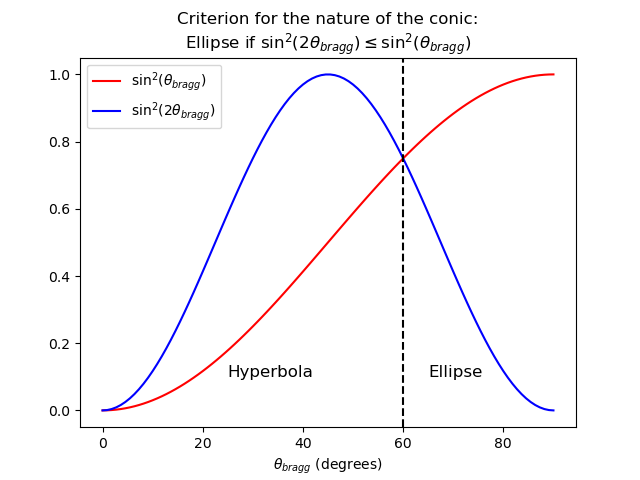
\includegraphics[width=0.6\linewidth]{Criterion_EllipseHyperbola.png}
    \caption{Criterion for the nature of the conic, for a tangential detector}
    \label{fig:boat1}
\end{center}
\end{figure}

Hence, for a tangential detector:
$$
\lt\{
	\begin{array}{lll}
        \theta_{bragg} < 60 \text{ degrees} \Rightarrow \text{ Hyperbola}\\
        \theta_{bragg} = 60 \text{ degrees} \Rightarrow \text{ Parabola}\\
        \theta_{bragg} > 60 \text{ degrees} \Rightarrow \text{ Ellipse}\\
	\end{array}
\rt.
$$

A similar computation can be done for a detector also on the rowland circle but
oriented in a direction perpendicular to the direction of the crystal, in this
case the results are:
$$
\lt\{
	\begin{array}{lll}
        \theta_{bragg} < 45 \text{ degrees} \Rightarrow \text{ Hyperbola}\\
        \theta_{bragg} = 45 \text{ degrees} \Rightarrow \text{ Parabola}\\
        \theta_{bragg} > 45 \text{ degrees} \Rightarrow \text{ Ellipse}\\
	\end{array}
\rt.
$$

\section{Parametric equation}

In our case, only the axes $(O, \ez)$, fixed by the crystal's summit and normal, is independent from the cone's angular opening $\theta$.
It makes sense to design an ad-hoc coordinate system centered on the ellipse's center $C$ to use its parameterized equation.

Knowing all geometrical parameters, it is possible to compute all points on the ellipse parameterizing them with $t$:
$$
\lt\{
	\begin{array}{lll}
		x_1 = a\cos(t)\\
		x_2 = x_2(C) + b\sin(t)
	\end{array}
\rt.
$$

\emph{BEWARE} : parameter $t$ is not the angle of the point with respect to the ellipse's center.

Now, we would like to parameterize the ellipse not with $t$ but with the angle $\beta$ with respect to the point $P$, because it is the physically relevant angle since it is taken with respect to the axis $(O, \ez)$ and relates to the impact point of the photon beam on the crystal's center. Also, it is the only common element to all ellipses.
The angle $\epsilon$ taken with respect to the center is not relevant because each ellipse has a different center.

In this perspective:
$$
\lt\{
	\begin{array}{lll}
		x_1 = l(\beta)\cos(\beta)\\
		x_2 = l(\beta)\sin(\beta)
	\end{array}
\rt.
$$

Keeping in mind that the ellipse is defined as:
$$
\frac{x_1^2}{a^2} + \frac{(x_2-x_2(C))^2}{b^2} = 1
$$

We can write:
$$
\begin{array}{lll}
	& l^2b^2\cos(\beta)^2 + a^2\lt(l^2\sin(\beta)^2 - 2lx_2(C)\sin(\beta) + x_2(C)^2\rt) = a^2b^2\\
	\Leftrightarrow
	& l^2\lt(b^2\cos(\beta)^2 + a^2\sin(\beta)^2\rt) - 2la^2x_2(C)\sin(\beta) + a^2x_2(C)^2 - a^2b^2 = 0
\end{array}
$$

Has solutions if:
$$
\begin{array}{lll}
	& \Delta = 4a^4x_2(C)^2\sin(\beta)^2 - 4\lt(b^2\cos(\beta)^2 + a^2\sin(\beta)^2\rt)\lt(a^2x_2(C)^2 - a^2b^2\rt) \geq 0\\
	\Leftrightarrow
	& \Delta = 4a^2\lt[a^2x_2(C)^2\sin(\beta)^2 - \lt(b^2\cos(\beta)^2 + a^2\sin(\beta)^2\rt)\lt(x_2(C)^2 - b^2\rt)\rt] \geq 0\\
	\Leftrightarrow
	& \Delta = 4a^2\lt[a^2x_2(C)^2\sin(\beta)^2 - b^2x_2(C)^2\cos(\beta)^2 - a^2x_2(C)^2\sin(\beta)^2 + b^4\cos(\beta)^2 + a^2b^2\sin(\beta)^2\rt] \geq 0\\
	\Leftrightarrow
	& \Delta = 4a^2\lt[-b^2x_2(C)^2\cos(\beta)^2 + b^4\cos(\beta)^2 + a^2b^2\sin(\beta)^2\rt] \geq 0\\
	\Leftrightarrow
	& \Delta = 4a^2b^2\lt[-x_2(C)^2\cos(\beta)^2 + b^2\cos(\beta)^2 + a^2\sin(\beta)^2\rt] \geq 0\\
\end{array}
$$

Which is equivalent to, keeping in mind that $b^2-a^2 = d_{CF}^2$:
$$
\begin{array}{lll}
	& \Delta = 4a^2b^2\lt[a^2 + \lt(b^2-a^2-x_2(C)^2\rt)\cos(\beta)^2\rt] \geq 0\\
	\Leftrightarrow
	& \lt(b^2-a^2-x_2(C)^2\rt)\cos(\beta)^2 \geq -a^2
	\Leftrightarrow
	& \lt(d_{CF}^2-x_2(C)^2\rt)\cos(\beta)^2 \geq -a^2
\end{array}
$$

If $d_{CF}^2-x_2(C)^2 \ geq 0$, this is true for all $\beta$ values, and this condition is met if:
$$
\begin{array}{lll}
	& b^2-a^2-x_2(C)^2 \geq 0\\
	\Leftrightarrow
	& \frac{Z_P^2}{\lt(\DD\rt)^2}\lt(\sin(\theta)^2\cos(\psi)^2\cos(\theta)^2 - \sin(\theta)^2\cos(\psi)^2\cos(\theta)^2 + \sin(\theta)^2\cos(\psi)^2\sin(\psi)^2 - \sin(\psi)^2\sin(\theta)^4\rt) \geq 0\\
	\Leftrightarrow
	& \sin(\theta)^2\sin(\psi)^2\lt(\cos(\psi)^2 -\sin(\theta)^2\rt) \geq 0
\end{array}
$$

Which is true if we have an ellipse, which is the only case of interest.
Hence $\Delta=4a^2b^2\lt[a^2 + \lt(b^2-a^2-x_2(C)^2\rt)\cos(\beta)^2\rt] \geq 0$, so:
$$
\begin{array}{lll}
	& l_{1,2} = \frac{2a^2x_2(C)\sin(\beta) \pm \sqrt{\Delta}}{2\lt(b^2\cos(\beta)^2 + a^2\sin(\beta)^2\rt)}\\
	\Leftrightarrow
	& l_{1,2} = \frac{a^2x_2(C)\sin(\beta) \pm ab\sqrt{a^2 + \lt(b^2-a^2-x_2(C)^2\rt)\cos(\beta)^2}}{b^2\cos(\beta)^2 + a^2\sin(\beta)^2}\\
\end{array}
$$

And we only want the positive solution:
$$
l = \frac{a^2x_2(C)\sin(\beta) + ab\sqrt{a^2 + \lt(b^2-a^2-x_2(C)^2\rt)\cos(\beta)^2}}{b^2\cos(\beta)^2 + a^2\sin(\beta)^2}
$$




\subsection{From bragg angle and parameter to local cartesian coordinates}

Keep in mind that the frame $(P, \ei, \et)$ is, by definition aligned on the minor and major axes of the ellipse.
Hence, for an arbitrary frame $(R, \ud{e}_i, \ud{e}_j)$ on plane $P_1$, translated and rotated by $\alpha$ with respect to $(P, \ei, \et)$:

$$
\lt\{
	\begin{array}{lll}
		\ud{e}_i = \cos(\alpha)\ei + \sin(\alpha)\et\\
		\ud{e}_j = -\sin(\alpha)\ei + \cos(\alpha)\et\\
		\ei = \cos(\alpha)\ud{e_i} - \sin(\alpha)\ud{e}_j
		\et = \sin(\alpha)\ud{e_i} + \cos(\alpha)\ud{e}_j
	\end{array}
\rt.
$$

Or, in coordinate tranforms:
$$
\lt\{
	\begin{array}{lll}
		x_1 = x_1(R) + x_i\cos(\alpha) - x_j\sin(\alpha)\\
		x_2 = x_2(R) + x_i\sin(\alpha) + x_j\cos(\alpha)\\
		x_i = (x_1-x_1(R))\cos(\alpha) + (x_2-x_2(R))\sin(\alpha)\\
		x_j = -(x_1-x_1(R))\sin(\alpha) + (x_2-x_2(R))\cos(\alpha)
	\end{array}
\rt.
$$

Hence:
$$
\lt\{
	\begin{array}{lll}
		x_i = \lt(a\cos(\epsilon)-x_1(R)\rt)\cos(\alpha) + \lt(x_2(C)-x_2(R) + b\sin(\epsilon)\rt)\sin(\alpha)\\
		x_j = -\lt(a\cos(\epsilon)-x_1(R)\rt)\sin(\alpha) + \lt(x_2(C)-x_2(R) + b\sin(\epsilon)\rt)\cos(\alpha)
	\end{array}
\rt.
$$

But
$$
\lt\{
	\begin{array}{lll}
		\|\ud{PM}\|^2 = x_1^2 + x_2^2 = \\
		x_1 = \|\ud{PM}\|\cos(\beta)\\
		x_2 = \|\ud{PM}\|\sin(\beta)
	\end{array}
\rt.
$$



\subsection{From local cartesian coordinates to bragg angle}

Knowing $(x_i, x_j)$ and all geometric parameters, we now want to derive $(\theta, \epsilon)$.

From the previous equation, we can write:
$$
\lt\{
	\begin{array}{lll}
        x_i\cos(\alpha) - x_j\sin(\alpha) = a\cos(\epsilon)-x_1(R) & (1)\\
        x_i\sin(\alpha) + x_j\cos(\alpha) = x_2(C)-x_2(R) + b\sin(\epsilon) &
        (2)
	\end{array}
\rt.
$$

The dependency in $\theta$ is hidden in the expressions of $a$, $b$ and
$x_2(C)$.

By squaring and summing, it is possible to get rid of the $\epsilon$
dependency:
$$
\lt\{
	\begin{array}{lll}
        a^2\cos(\epsilon)^2 = \lt(x_i\cos(\alpha) - x_j\sin(\alpha) +
        x_1(R)\rt)^2\\
        b^2\sin(\epsilon)^2 = \lt(x_i\sin(\alpha) + x_j\cos(\alpha) - x_2(C) +
        x_2(R)\rt)^2
	\end{array}
\rt.
$$

Hence, keeping in mind that $a^2 = b^2\frac{\DD}{\cos(\theta)^2}$ and re-using the definitions of $x_1$ and $x_2$ which do not depend on the unknowns $(\theta, \epsilon)$:
$$
\begin{array}{lllll}
	& b^2 & = & \frac{\cos(\theta)^2}{\DD}x_1^2 + \lt(x_2 - x_2(C)\rt)^2\\
    \Leftrightarrow
    & b^2\lt(\DD\rt) & = & \cos(\theta)^2x_1^2 + \lt(\DD\rt)\lt(x_2^2 - 2x_2x_2(C) + x_2(C)^2\rt)\\
    \Leftrightarrow
    &  Z_P^2\frac{\sin(\theta)^2\cos(\psi)^2\cos(\theta)^2}{\DD} & = & \cos(\theta)^2x_1^2 + \lt(\DD\rt)\lt(x_2^2 - 2x_2x_2(C) + x_2(C)^2\rt)\\
    \Leftrightarrow
    &  Z_P^2\frac{\sin(\theta)^2\cos(\psi)^2\cos(\theta)^2}{\DD} & = & \cos(\theta)^2\lt(x_1^2+x_2^2\rt) - \sin(\psi)^2x_2^2 - \lt(\DD\rt)\lt(2x_2x_2(C) - x_2(C)^2\rt)\\
    \Leftrightarrow
    &  Z_P^2\sin(\theta)^2\cos(\psi)^2\cos(\theta)^2 & = & \cos(\theta)^2\lt(\DD\rt)\lt(x_1^2+x_2^2\rt) - \sin(\psi)^2\lt(\DD\rt)x_2^2\\
    \Leftrightarrow
    & & & - \lt(\DD\rt)^2\lt(2x_2x_2(C) - x_2(C)^2\rt)\\
    \Leftrightarrow
    &  Z_P^2\sin(\theta)^2\cos(\psi)^2\cos(\theta)^2 & = &\cos(\theta)^4\lt(x_1^2+x_2^2\rt) - \cos(\theta)^2\sin(\psi)^2\lt(x_1^2+2x_2^2\rt) + \sin(\psi)^4x_2^2\\
    & & & - \lt(\DD\rt)^2\lt(2x_2x_2(C) - x_2(C)^2\rt)\\
    \Leftrightarrow
    &  Z_P^2\sin(\theta)^2\cos(\psi)^2\cos(\theta)^2 & = & \cos(\theta)^4\lt(x_1^2+x_2^2\rt) - \cos(\theta)^2\sin(\psi)^2\lt(x_1^2+2x_2^2\rt) + \sin(\psi)^4x_2^2\\
    & & & - \lt[2x_2Z_P\sin(\psi)\sin(\theta)^2\lt(\DD\rt) - Z_P^2\sin(\psi)^2\sin(\theta)^4\rt]\\
    \Leftrightarrow
    &  Z_P^2\cos(\psi)^2\lt(\cos(\theta)^2-\cos(\theta)^4\rt) & = &\cos(\theta)^4\lt(x_1^2+x_2^2\rt) - \cos(\theta)^2\sin(\psi)^2\lt(x_1^2+2x_2^2\rt) + \sin(\psi)^4x_2^2\\
    & & & - 2x_2Z_P\sin(\psi)\sin(\theta)^2\lt(\DD\rt)\\
    & & & + Z_P^2\sin(\psi)^2\lt(1-2\cos(\theta)^2+\cos(\theta)^4\rt)\\
    \Leftrightarrow
    &  Z_P^2\cos(\psi)^2\lt(\cos(\theta)^2-\cos(\theta)^4\rt) & = &\cos(\theta)^4\lt(x_1^2+x_2^2\rt) - \cos(\theta)^2\sin(\psi)^2\lt(x_1^2+2x_2^2\rt) + \sin(\psi)^4x_2^2\\
    & & & - 2x_2Z_P\sin(\psi)\lt(\cos(\theta)^2 - \cos(\theta)^4 - \sin(\psi)^2\lt(1-\cos(\theta)^2\rt)\rt)\\
    & & & + Z_P^2\sin(\psi)^2\lt(1-2\cos(\theta)^2+\cos(\theta)^4\rt)
\end{array}
$$

Then introducing $X = \cos(\theta)^2$:
$$
\begin{array}{lllll}
	& b^2 & = & \frac{\cos(\theta)^2}{\DD}x_1^2 + \lt(x_2 - x_2(C)\rt)^2\\
    \Leftrightarrow
    &  Z_P^2\cos(\psi)^2\lt(X-X^2\rt) & = & X^2\lt(x_1^2+x_2^2\rt) - X\sin(\psi)^2\lt(x_1^2+2x_2^2\rt) + \sin(\psi)^4x_2^2\\
    & & & - 2x_2Z_P\sin(\psi)\lt(X - X^2 - \sin(\psi)^2 + X\sin(\psi)^2\rt)\\
    & & & + Z_P^2\sin(\psi)^2\lt(1 - 2X + X^2\rt)
\end{array}
$$

Which boils down to:
$$
\begin{array}{lllll}
    & 0 & = & X^2\lt[ x_1^2+x_2^2 + 2x_2Z_P\sin(\psi) + Z_P^2\sin(\psi)^2 + Z_P^2\cos(\psi)^2 \rt]\\
    & & & + X\lt[ -\sin(\psi)^2\lt(x_1^2+2x_2^2\rt) - \lt(1+\sin(\psi)^2\rt)2x_2Z_P\sin(\psi) - 2Z_P^2\sin(\psi)^2 - Z_P^2\cos(\psi)^2\rt]\\
    & & & + \sin(\psi)^4x_2^2 + 2x_2Z_P\sin(\psi)^3 + Z_P^2\sin(\psi)^2\\
    \Leftrightarrow
    & 0 & = & X^2\lt[ x_1^2 + \lt(x_2 + Z_P\sin(\psi)\rt)^2 + Z_P^2\cos(\psi)^2 \rt]\\
    & & & + X\lt[ -\sin(\psi)^2\lt(x_1^2+2x_2^2\rt) - \lt(1+\sin(\psi)^2\rt)2x_2Z_P\sin(\psi) - 2Z_P^2\sin(\psi)^2 - Z_P^2\cos(\psi)^2\rt]\\
    & & & + \sin(\psi)^2\lt(\sin(\psi)^2x_2^2 + 2x_2Z_P\sin(\psi) + Z_P^2\rt)\\
    \Leftrightarrow
    & 0 & = & X^2\lt[ x_1^2 + \lt(x_2 + Z_P\sin(\psi)\rt)^2 + Z_P^2\cos(\psi)^2 \rt]\\
    & & & - X\lt[ \sin(\psi)^2\lt(x_1^2+2x_2^2\rt) + \lt(1+\sin(\psi)^2\rt)2x_2Z_P\sin(\psi) + 2Z_P^2\sin(\psi)^2 + Z_P^2\cos(\psi)^2\rt]\\
    & & & + \sin(\psi)^2\lt(x_2\sin(\psi) + Z_P\rt)\\
    \Leftrightarrow
    & 0 & = & X^2\lt[ x_1^2 + \lt(x_2 + Z_P\sin(\psi)\rt)^2 + Z_P^2\cos(\psi)^2 \rt]\\
    & & & - X\lt[ \sin(\psi)^2\lt(x_1^2+x_2^2\rt) + x_2^2\sin(\psi)^2 + 2x_2Z_P\sin(\psi) + 2x_2Z_P\sin(\psi)^3 + Z_P^2 + Z_P^2\sin(\psi)^2\rt]\\
    & & & + \sin(\psi)^2\lt(x_2\sin(\psi) + Z_P\rt)\\
    \Leftrightarrow
    & 0 & = & X^2\lt[ x_1^2 + \lt(x_2 + Z_P\sin(\psi)\rt)^2 + Z_P^2 - Z_P^2\sin(\psi)^2 \rt]\\
    & & & - X\lt[ \sin(\psi)^2\lt(x_1^2+x_2^2\rt) + \lt(x_2\sin(\psi) + Z_P\rt)^2 + Z_P\sin(\psi)^2\lt(2x_2\sin(\psi) + Z_P\rt)\rt]\\
    & & & + \sin(\psi)^2\lt(x_2\sin(\psi) + Z_P\rt)\\
    \Leftrightarrow
    & 0 & = & X^2\lt[ x_1^2 + x_2^2 + \lt(x_2\sin(\psi) + Z_P\rt)^2 - x_2^2\sin(\psi)^2 \rt]\\
    & & & - X\lt[ \sin(\psi)^2\lt(x_1^2+x_2^2\rt) + \lt(x_2\sin(\psi) + Z_P\rt)^2 + Z_P\sin(\psi)^2\lt(2x_2\sin(\psi) + Z_P\rt)\rt]\\
    & & & + \sin(\psi)^2\lt(x_2\sin(\psi) + Z_P\rt)\\
    \Leftrightarrow
    & 0 & = & AX^2 - BX + C
\end{array}
$$

With:

$$
\lt\{
	\begin{array}{lll}
		A = x_1^2 + x_2^2 + \lt(x_2\sin(\psi) + Z_P\rt)^2 - x_2^2\sin(\psi)^2\\
		B = \sin(\psi)^2\lt(x_1^2+x_2^2\rt) + \lt(x_2\sin(\psi) + Z_P\rt)^2 + Z_P\sin(\psi)^2\lt(2x_2\sin(\psi) + Z_P\rt)\\
		C = \sin(\psi)^2\lt(x_2\sin(\psi) + Z_P\rt)
	\end{array}
\rt.
$$

Solutions exist if:
$$
\begin{array}{lllll}
    & \Delta & \geq & 0\\
    \Leftrightarrow
    & B^2 - 4AC & \geq & 0\\
\end{array}
$$

In which case, only solutions in $\lt[0,1\rt]$ are acceptable:
$$
\cos(\theta)^2 = \frac{B \pm \sqrt(\Delta)}{2A} \in \lt[0,1\rt]
$$

And by definition, $\theta \in \lt[0,\frac{\pi}{2}\rt]$, hence $\cos(\theta)\geq0$ and:
$$
\theta = \arccos\lt(\sqrt{\frac{B \pm \sqrt(\Delta)}{2A}}\rt)
$$

\subsubsection{Alternative method for $\theta$}

By definition:
$$
\underline{OM}.\ez = \cos(\theta)\|OM\|
$$

And:
$$
\begin{array}{lllll}
	\underline{OM} 	& = & \underline{OP} + \underline{PR} + \underline{RM}\\
			& = & \\
\end{array}
$$

\newpage
\section{Generalization}

This time, the crystal of curvature radius $R$ has center $C$ of coordinates $(x_C, y_C, z_C)$ in the tokamak's frame $(O, \ex, \ey, \ez)$.\\
The direct orthonormal systems are:

\begin{figure}[hbt]
	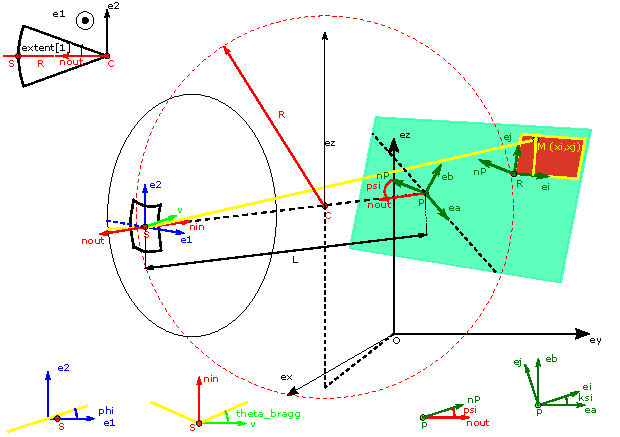
\includegraphics[width=\linewidth]{SpectroX2D_Crystal.pdf}
	\caption{Definition of the generilazed geometry}
	\label{fig:sketch}
\end{figure}


$$
\lt\{
	\begin{array}{lll}
		(O, \ex, \ey, \ez)\\
		(C, \nout, \e{1}, \e{2})\\
		(P, \np, \e{a}, \e{b})\\
		(R, \np, \e{i}, \e{j})
	\end{array}
\rt.
$$

\subsection{Direct problem}

We know all geometrical parameters, in particular, we know:
$$
\lt\{
	\begin{array}{lll}
		\ud{OC} = x(C)\ex + y(C)\ey + z(C)\ez\\
		\ud{CS} = R\nout\\
		\ud{SP} = -L\nout\\
		\ud{PR} = x_a(R)\e{a} + x_b(R)\e{b}\\
		\ud{RM} = x_i\e{i} + x_j\e{j}
	\end{array}
\rt.
$$






\appendix
\chapter{Appendices}

\section{Section}
\subsection{Subsection}

\end{document}
